The results of the 24-hour latency test indicate that there is a significant delay between the real agents located in Copenhagen, Denmark and the cloud provider data center located in Council Bluffs, Iowa, United States. The distance between these locations is roughly 7500km, which may contribute to the observed delays. During the test, an ICMP package with 32 bytes of data was sent every minute to the cloud broker endpoint, and the Round Trip Time (RTT) was measured. The results of this test can be viewed in Figure \ref{fig:ping}. RTT ping test is a method used to measure the time it takes for a packet of data to travel from a source device to a destination device and for the response to travel back to the source device.

\begin{figure}[H]
    \centering
    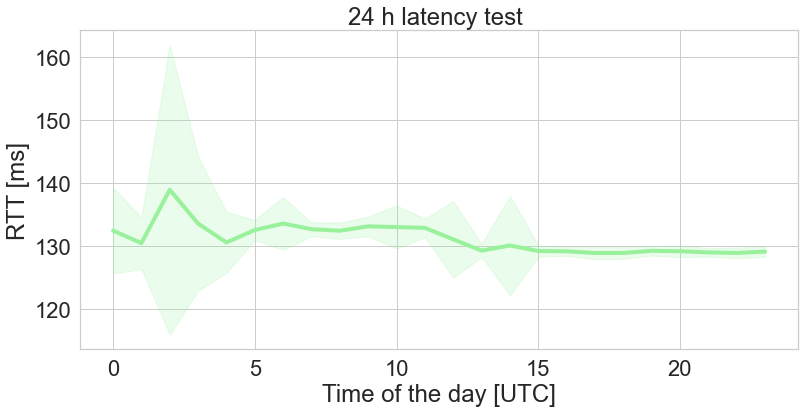
\includegraphics[width=0.8\textwidth]{pictures/ping.png}
    \caption{RTT time}
    \label{fig:ping}
\end{figure}

The results of the test revealed an average RTT of 131 milliseconds, with a minimum RTT of 126 milliseconds, a maximum RTT of 236 milliseconds, and a standard deviation of 6 milliseconds over the entire test period. The largest standard deviation was observed between 1 and 4 AM UTC.